\documentclass{article}
\usepackage{amsmath,amssymb,amsthm} % AMS styles for extra equation formatting
\usepackage{graphicx} % for including graphics files
\usepackage{subfig} % for subfigures
\usepackage[numbers,sort]{natbib} % for better references control
\usepackage{hyperref} % for hyperlinks within the paper and references
\usepackage{fontspec}  % Allows for system fonts
\usepackage[top=2cm, bottom=2cm, left=2cm, right=2cm]{geometry}  % Set margins on all sides
\usepackage{setspace} % for line spacing
\usepackage{appendix} % for the appendices
\usepackage{listings} % for code
\usepackage{xcolor} % for color
\usepackage{url,textcomp}
\usepackage{matlab-prettifier}
\usepackage{tabularx}
%%%%%%%%%%%%%%%%%%%%%%%%%%%%%%%%%%%%%%%%%%%%%%%%%%%%%%%%%%%%%%%%%%%%%%%%%%%%%%

\hypersetup{colorlinks=true, linkcolor=blue,  anchorcolor=blue,
citecolor=blue, filecolor=blue, menucolor=blue, pagecolor=blue,
urlcolor=blue}

%%%%%%%%%%%%%%%%%%%%%%%%%%%%%%%%%%%%%%%%%%%%%%%%%%%%%%%%%%%%%%%%%%%%%%%%%%%%%%

\newcommand{\todo}[1]{\vspace{5 mm}\par \noindent
\marginpar{\textsc{Todo}}
\framebox{\begin{minipage}[c]{0.90 \textwidth}
\tt \flushleft #1 \end{minipage}}\vspace{5 mm}\par}
\newcommand{\setParDis}{\setlength {\parskip} {0.2cm} } % for 0.3cm spacing
\newcommand{\setParDef}{\setlength {\parskip} {0pt} } % for 0 spacing

%%%%%%%%%%%%%%%%%%%%%%%%%%%%%%%%%%%%%%%%%%%%%%%%%%%%%%%%%%%%%%%%%%%%%%%%%%%%%%

\graphicspath{{graphics/}}

\newtheorem{theorem}{Theorem}[section]
\newtheorem{proposition}[theorem]{Proposition}
\newtheorem{lemma}[theorem]{Lemma}
\newtheorem{corollary}[theorem]{Corollary}
\newtheorem{definition}[theorem]{Definition}

%\renewcommand{\qedsymbol}{$\blacksquare$} % for filled square at end of proof
%\numberwithin{equation}{section} % for the 1.1, 1.2 equation number style
%\setlength{\parindent}{0em} % don't indent paragraphs
%\setlength{\parskip}{1em} % add spacing between paragraphs
%\linespread{1.6} % double-spacing

\setmainfont{Arial}
% \doublespacing
\onehalfspacing
\setcounter{secnumdepth}{3}

%%%%%%%%%%%%%%%%%%%%%%%%%%%%%%%%%%%%%%%%%%%%%%%%%%%%%%%%%%%%%%%%%%%%%%%%%%%%%%

\begin{document}

\title{%
Report for Speech Recognition \\
\large\itshape{EEEM030 - Speech Recognition - Group Assignment 2}}
\author{\normalsize\slshape{Xiaoguang Liang, Tofarati Onatunde, and Zeyad Adelmonem}}
\date{\normalsize\slshape\today}
\maketitle


% Suppress any floats (figures, tables) from appearing on the next page
\suppressfloats

\tableofcontents

\begin{abstract}
Abstract
This report presents the implementation of a speech recognition system based on a Hidden Markov Model (HMM) for isolated word recognition. Utilizing precomputed Mel-Frequency Cepstral Coefficients (MFCCs) as features, the system incorporates feature normalization, parameter initialization for the HMM, sequence decoding via the Viterbi algorithm, and comprehensive evaluation metrics. The system’s performance is assessed through recognition error rate (RER) and a confusion matrix, providing insights into its effectiveness in identifying words from a limited vocabulary. The implementation demonstrates the application of HMMs in speech recognition and highlights the impact of key steps such as initialization and decoding on system accuracy.

\end{abstract}

%%%%%%%%%%%%%%%%%%%%%%%%%%%%%%%%%%%%%%%%%%%%%%%%%%%%%%%%%%%%%%%%%%%%%%%%%%%%%%

\section{Introduction}
\setParDis
This report outlines the implementation of a speech recognizer using a Hidden Markov Model (HMM). The model was developed to process precomputed Mel-Frequency Cepstral Coefficients (MFCCs) for isolated word recognition. The implementation involves feature normalization, initialization of HMM parameters, decoding using the Viterbi algorithm, and evaluation metrics, including recognition error rate and a confusion matrix.

The primary goal of this assignment is to implement a speech recognizer based on a Hidden Markov Model (HMM) that can identify isolated words from a small vocabulary using Mel-Frequency Cepstral Coefficients (MFCCs) as features. The system aims to process precomputed MFCCs, apply normalization, initialize HMM parameters, and use the Viterbi algorithm to decode the sequence of states. Performance is evaluated using the Recognition Error Rate (RER) and a Confusion Matrix.

This report is structured as follows: \textit{Section 2} is to extract MFCC acoustic features. \textit{Section 3} indroduces the model initialization for a set of prototype HMMs for each word in the vooabulary. \textit{Section 4} explores training the HMMs with the training data in detail. \textit{Section 5} evaluates the recognizer on the development set and the evaluation set. \textit{Section 6} explores data augmentation to improve the performance of HMM. Finally, conclusions are drawn in \textit{Section 7}.

%%%%%%%%%%%%%%%%%%%%%%%%%%%%%%%%%%%%%%%%%%%%%%%%%%%%%%%%%%%%%%%%%%%%%%%%%%%%%%

\section{MFCC acoustic features}


\section{Model initialization}


\subsection{Paremeters of HMM initialization}

Model initialization represents a fundamental stage in the training of Hidden Markov Models (HMMs). The efficacy of training algorithms such as the Baum-Welch algorithm is contingent upon the initialisation of model parameters in an optimal manner. These parameters encompass the initial state probabilities, represented by the symbol $\pi$, the state transition probabilities $A$, and the observation probabilities $B$. The implementation of an appropriate initialisation strategy provides a robust foundation for optimisation, whilst simultaneously preventing the convergence to suboptimal solutions. 

\paragraph{Initial State Probabilities $\Pi$:}
	 $\Pi = [\pi_1, \pi_2, \dots, \pi_N]$ represents the probability of starting in each state $i$ , where  $N$ is the number of states.
As indicated in the assignment document, the initial value of $\Pi$ is provided as follows:
\begin{equation}
\label{eqn:pi}
\pi_i = \begin{bmatrix}
 	1 & 0 & 0 & 0 & 0 & 0 & 0 & 0
 \end{bmatrix}
\end{equation}

\paragraph{State Transition Probabilities $A$:}
 $A = [a_{ij}]$  represents the probability of transitioning from state $i$ to state $j$, satisfying $\sum_{j=1}^N a_{ij} = 1$  for all $i$.
Here, initial $A$ is provided in the assigment document:
\begin{equation}
\label{eqn:A}
a_{ij} = \begin{bmatrix}
 	0.8 & 0.2 & 0 & 0 & 0 & 0 & 0 & 0 \\
 	0 & 0.8 & 0.2 & 0 & 0 & 0 & 0 & 0 \\
 	0 & 0 & 0.8 & 0.2 & 0 & 0 & 0 & 0 \\
 	0 & 0 & 0 & 0.8 & 0.2 & 0 & 0 & 0 \\
 	0 & 0 & 0 & 0 & 0.8 & 0.2 & 0 & 0 \\
 	0 & 0 & 0 & 0 & 0 & 0.8 & 0.2 & 0 \\
 	0 & 0 & 0 & 0 & 0 & 0 & 0.8 & 0.2 \\
 	0 & 0 & 0 & 0 & 0 & 0 & 0 & 0.8
 \end{bmatrix}
\end{equation}

\paragraph{Observation Probabilities $B$:}
 $B$ represents the probability of observing data given a state. For continuous observations, this is computed using a multivariate Gaussian probability density function $PDF$.
 
 The observation probability for a given state $i$ and observation $x$ is defined as:
\begin{equation}
B_i(x) = \frac{1}{(2\pi)^{d/2} |\Sigma_i|^{1/2}} e^{-\frac{1}{2}(x - \mu_i)^T \Sigma_i^{-1} (x - \mu_i)}
\end{equation}

where:
\begin{itemize}
\item $\mu_i$ is the mean vector for state  i ,
\item $\Sigma_i$ is the covariance matrix for state  i ,
\item $d$ is the dimensionality of the observation vector.
\end{itemize}

In practice:
\begin{itemize}
\item $\mu_i$ can be initialized as the global mean of the observations.
\item $\Sigma_i$ can be initialized as a diagonal matrix where diagonal entries are the variances of the clustered observations.
\end{itemize}

\subsection{Initializaton for Multivariate Gaussian PDF}

In models with multivariate Gaussian probability density functions (PDFs), the initialisation of model parameters is of critical importance for the success of the training process, particularly when using iterative algorithms such as the Baum-Welch algorithm. The process of initialization provides the model with initial estimates for the emission probabilities, which are represented as Gaussian distributions, as well as the transition probabilities and initial state probabilities.

The initialisation of the multivariate Gaussian PDF necessitates the estimation of the mean vector, designated as $\mu$, and the covariance matrix, designated as $\Sigma$, for each state within the HMM. These parameters serve to characterise the probability distribution of the observed data within each state.

\subsubsection{Segments splitting for data}
Divide the length of the feature data evenly into $N$ parts, where $N = 8$, representing the number of hidden states. This converts the training samples into an $8N\times13$matrix, facilitating the computation of the Multivariate Gaussian PDF.

\subsubsection{Calculation for mean}
As the quirement for this assigment, to obtain a $13\times13$ mean matrix, the feature data should be splitted into $N$ segments. And then loop through each segment to calculate the mean. For a matrix $X$ of size $m \times n$, the mean of each row is:
\begin{equation}	
\mu_i = \frac{1}{n} \sum_{j=1}^{n} X_{i,j}, \quad i = 1, 2, \ldots, m
\end{equation}

\subsubsection{Calculation for variance}
As the quirement for this assigment, to obtain the diagonal of the $13\times13$ covariance matrix, the feature data should be splitted into $N$ segments, same as the method of computing mean. And then loop through each segment to calculate the covariance matrix. For a matrix $X$ of size $m \times n$, the variance of each row is:
\begin{equation}	
Varrow(X) = \frac{1}{n} \sum{j=1}^n \left(X_{ij} - \mu_i\right)^2, \quad i = 1, 2, \dots, m
\end{equation}
where $\mu_i$ is the mean of the $i$-$th$ row.

\subsection{Normalization and regularization}
\paragraph{Normalization:} Normalize the input data to have zero mean and unit variance to ensure robust parameter estimation. In practice, Min-Max Normalization is implemented. Scales all elements to the range [0, 1] like this:
\begin{equation}
\text{Normalized Value} = \frac{\text{Value} - \text{Min}}{\text{Max} - \text{Min}}
\end{equation}

\paragraph{Regularization:} Regularizing the covariance matrix can prevent issues like singular matrices or overfitting. A small value epsilon is added to the diagonal elements of the covariance matrix:
\begin{equation}
\text{Regularized Matrix} = \text{Covariance Matrix} + \epsilon \cdot I
\end{equation}
where $I$ is the identity matrix.


\section{Model training with HMMs}


\section{Evaluation}

\subsection{Viterbi Algorithm}
The Viterbi algorithm is used for decoding the sequence of hidden states given the observation sequence. The algorithm uses dynamic programming to compute the maximum likelihood of the entire sequence by recursively calculating the most probable state at each time step.

\paragraph{Steps of the Viterbi Algorithm:}
\begin{enumerate}
\item Initialization: At time t=1, the probability of each state is computed using the initial state probabilities $\Pi$ and the emission probabilities $B$.
\item Recursion: For each subsequent time step t, the algorithm computes the maximum probability of each state by considering all transitions from previous states. This is done by combining the previous state’s probability and the transition probability.
\item Termination: After processing all time frames, the algorithm selects the state with the highest probability at the final time frame.
\item Backtracking: The state sequence is traced back using the back pointer matrix, which keeps track of the state transitions that led to the optimal path.
\end{enumerate}

\paragraph{Numerical Stability:}
To avoid underflow issues, probabilities are represented in logarithmic space. This ensures that the product of small probabilities does not result in numerical errors. Instead of multiplying probabilities, we add their logarithms.


\subsection{Evaluation on the development set}

\paragraph{Recognition error rate:} This is the percentage of misclassified predictions in the test set compared to the ground truth. The formula for RER is:
\begin{equation}
	Error Rate = \frac{Number of Incorrect Predictions}{Total Predictions}
\end{equation}

\paragraph{Confusion Matrix:} A confusion matrix is a table used to describe the performance of a classification model. Each row represents the true labels, while each column represents the predicted labels. It helps visualize the types of misclassifications made by the model.

In accordance with the specifications set forth in the assignment, the HMM model was trained for a total of 15 epochs. The error rates are calculated on the basis of the outputs of the Viterbi algorithm, and the resulting error rates on the development set are presented in the accompanying figure \ref{fig:error-rate} and the error rates data is in the Table \ref{table:error-rates}.

\begin{figure}[h]
\begin{center}
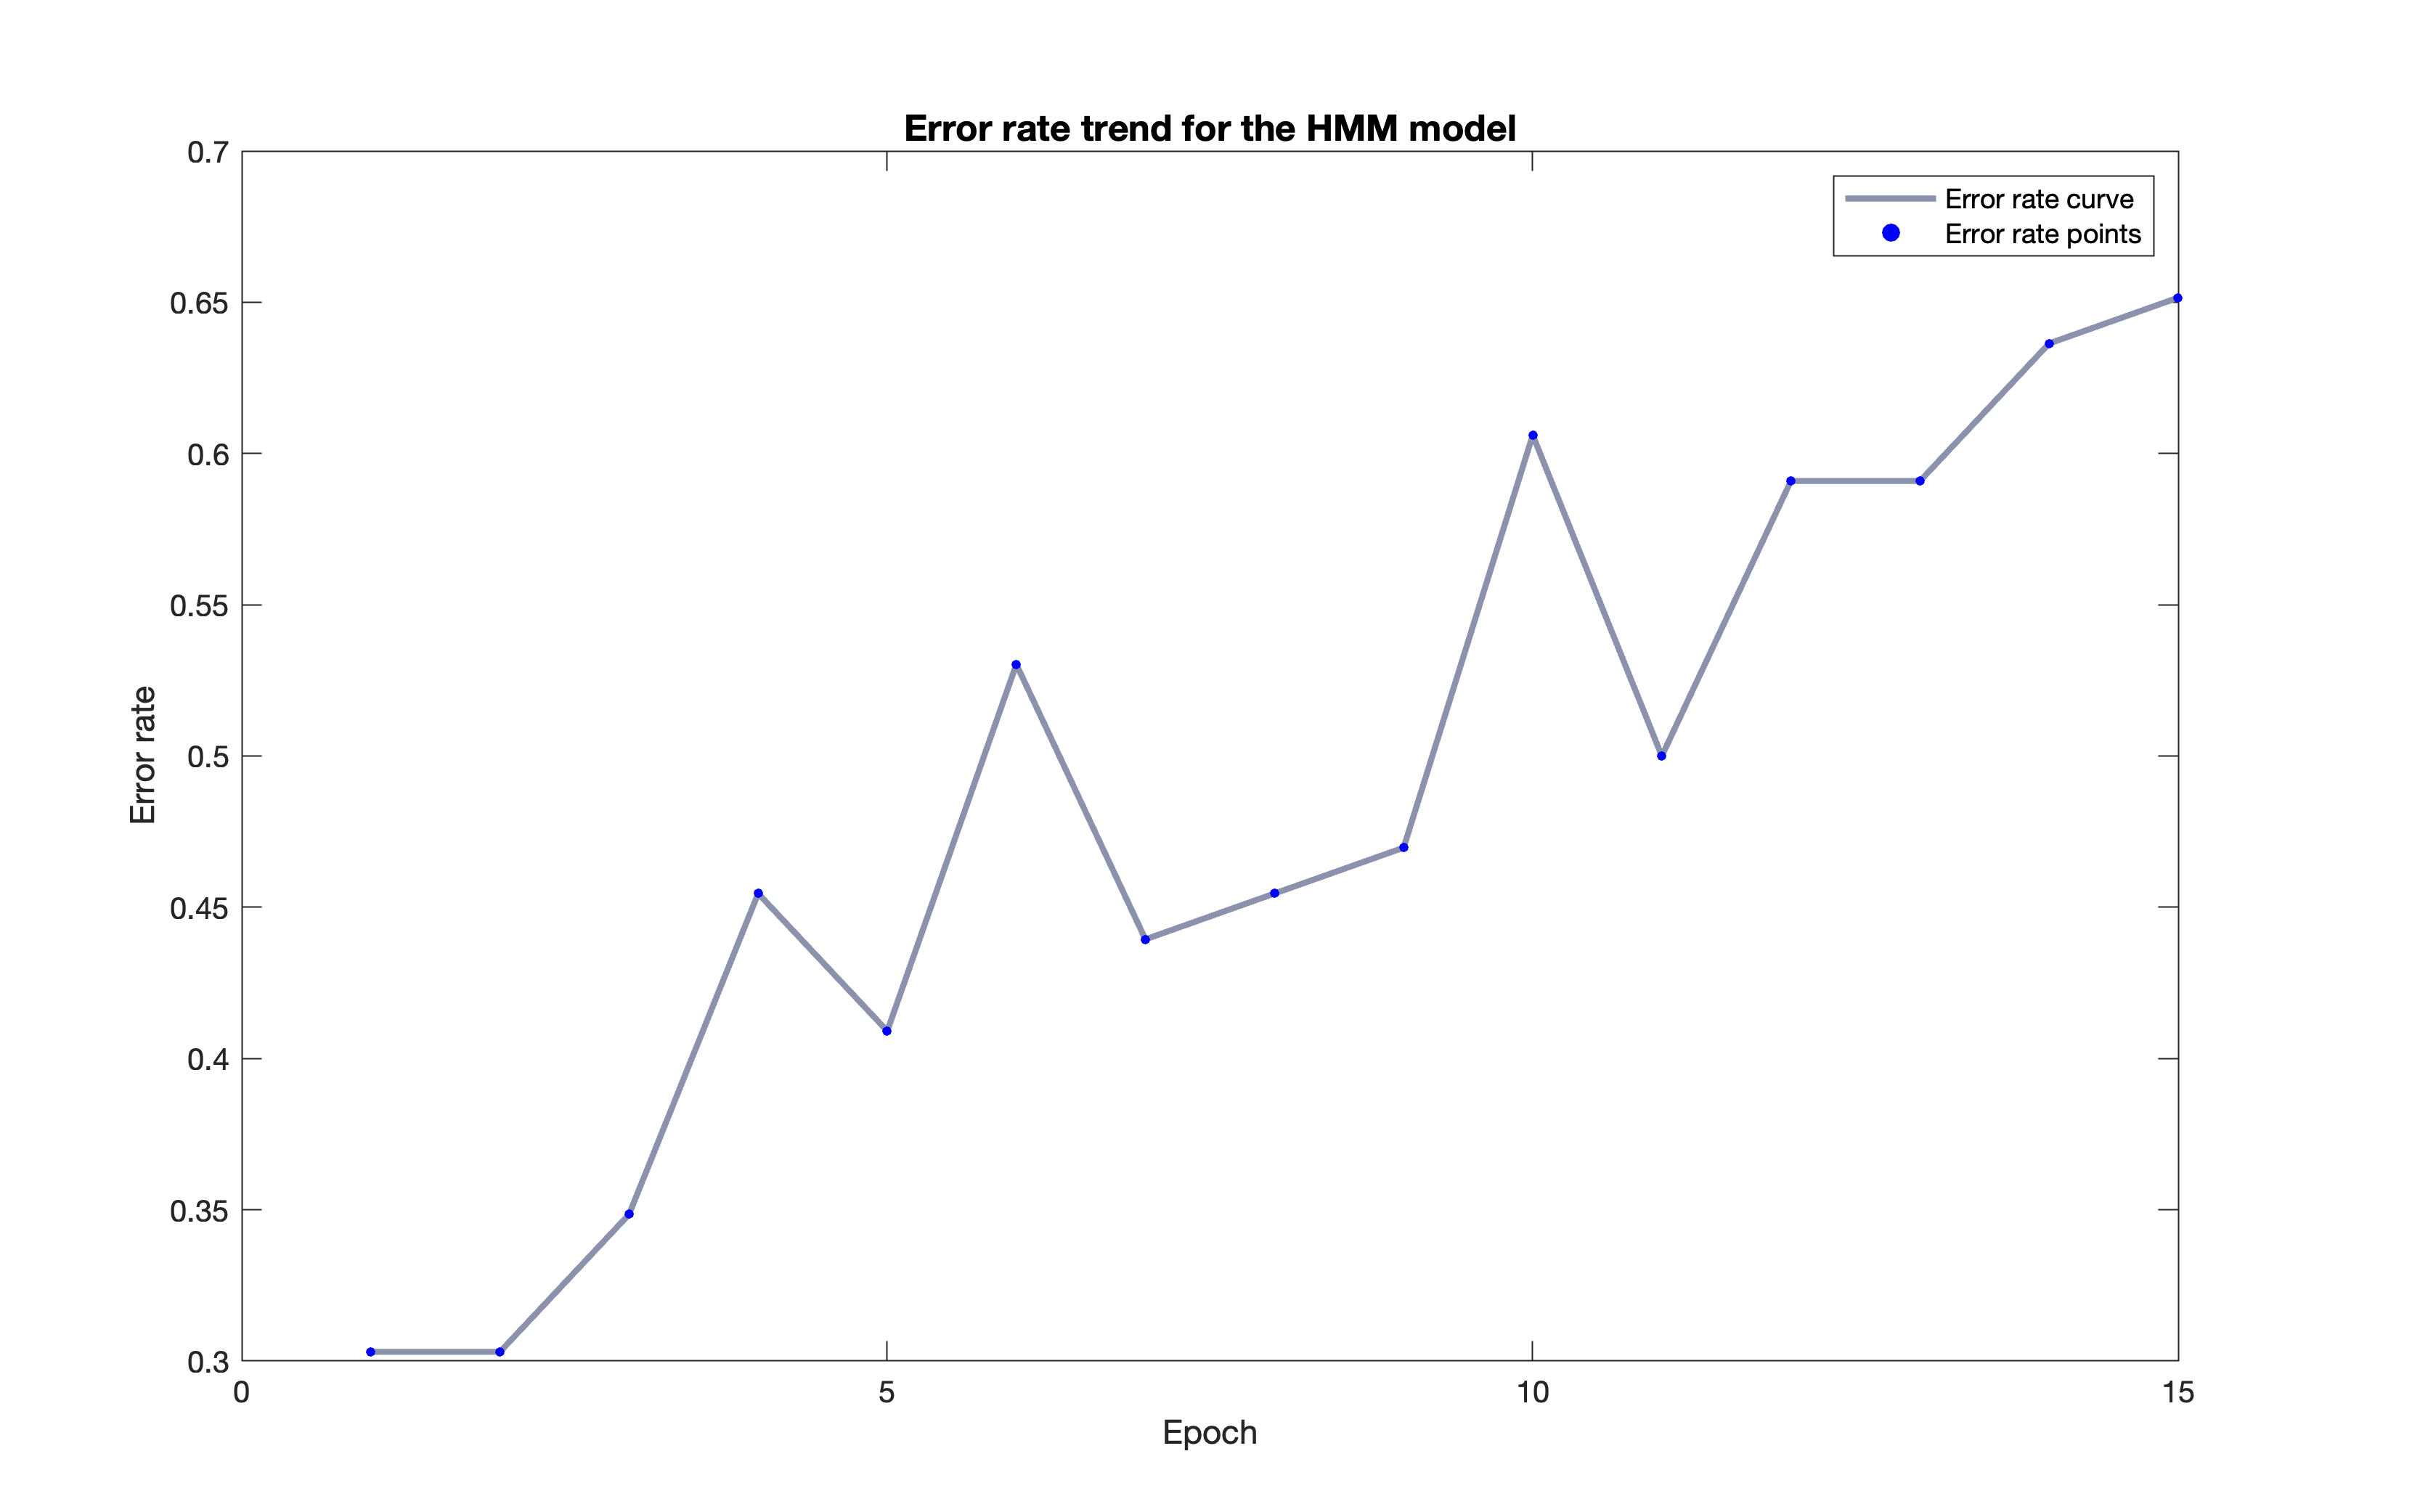
\includegraphics[width=\textwidth]{Error_rate_trend_for_HMM_model}
\end{center}
\caption{\label{fig:error-rate} Error rate trend for HMM model training on the development set.}
\end{figure}


\begin{table}[h]
\caption{Error rates for HMM model training on the development set} % title of Table
\centering % used for centering table
\label{table:error-rates}
{\large %
\begin{tabularx}{0.5\textwidth}[h]
 { 
  | >{\centering\arraybackslash}X 
  | >{\centering\arraybackslash}X | }
 \hline
 Epoch & Error rate\\
 \hline
 1  & 0.393939  \\
 \hline
 2  & 0.393939  \\
 \hline
 3  & 0.5 \\
 \hline
 4  & 0.530303  \\
 \hline
 5  & 0.424242  \\
 \hline
 6  & 0.5  \\
 \hline
 7  & 0.409091  \\
 \hline
 8  & 0.454545  \\
 \hline
 9  & 0.393939 \\
 \hline
 10  & 0.424242  \\
 \hline
 11  & 0.363636  \\
 \hline
 12  & 0.424242  \\
 \hline
 13  & 0.424242 \\
 \hline
 14  & 0.515152  \\
 \hline
 15  & 0.424242  \\
 \hline
\end{tabularx}
}%
\end{table}



\subsection{Evaluation on the evaluation set}

The evaluation is conducted on the evaluation set provided in the assignment. In order to ascertain the accuracy of the HMM model, the maximum cumulative likelihoods are initially calculated using the Viterbi algorithm. Subsequently, the accuracy is calculated based on the output of the Viterbi algorithm. The most optimal HMM model exhibits an accuracy of 0.318182 on the evaluation set. The equation for calculating accuracy is as follows:
\begin{equation}
	Accuracy = \frac{Number of Correct Predictions}{Total Predictions}
\end{equation}

The recognition outputs should be evaluated and a confusion matrix generated. The corresponding confusion matrix is presented in graphical form in Figure \ref{fig:confusion-matrix}.

\begin{figure}[h]
\begin{center}
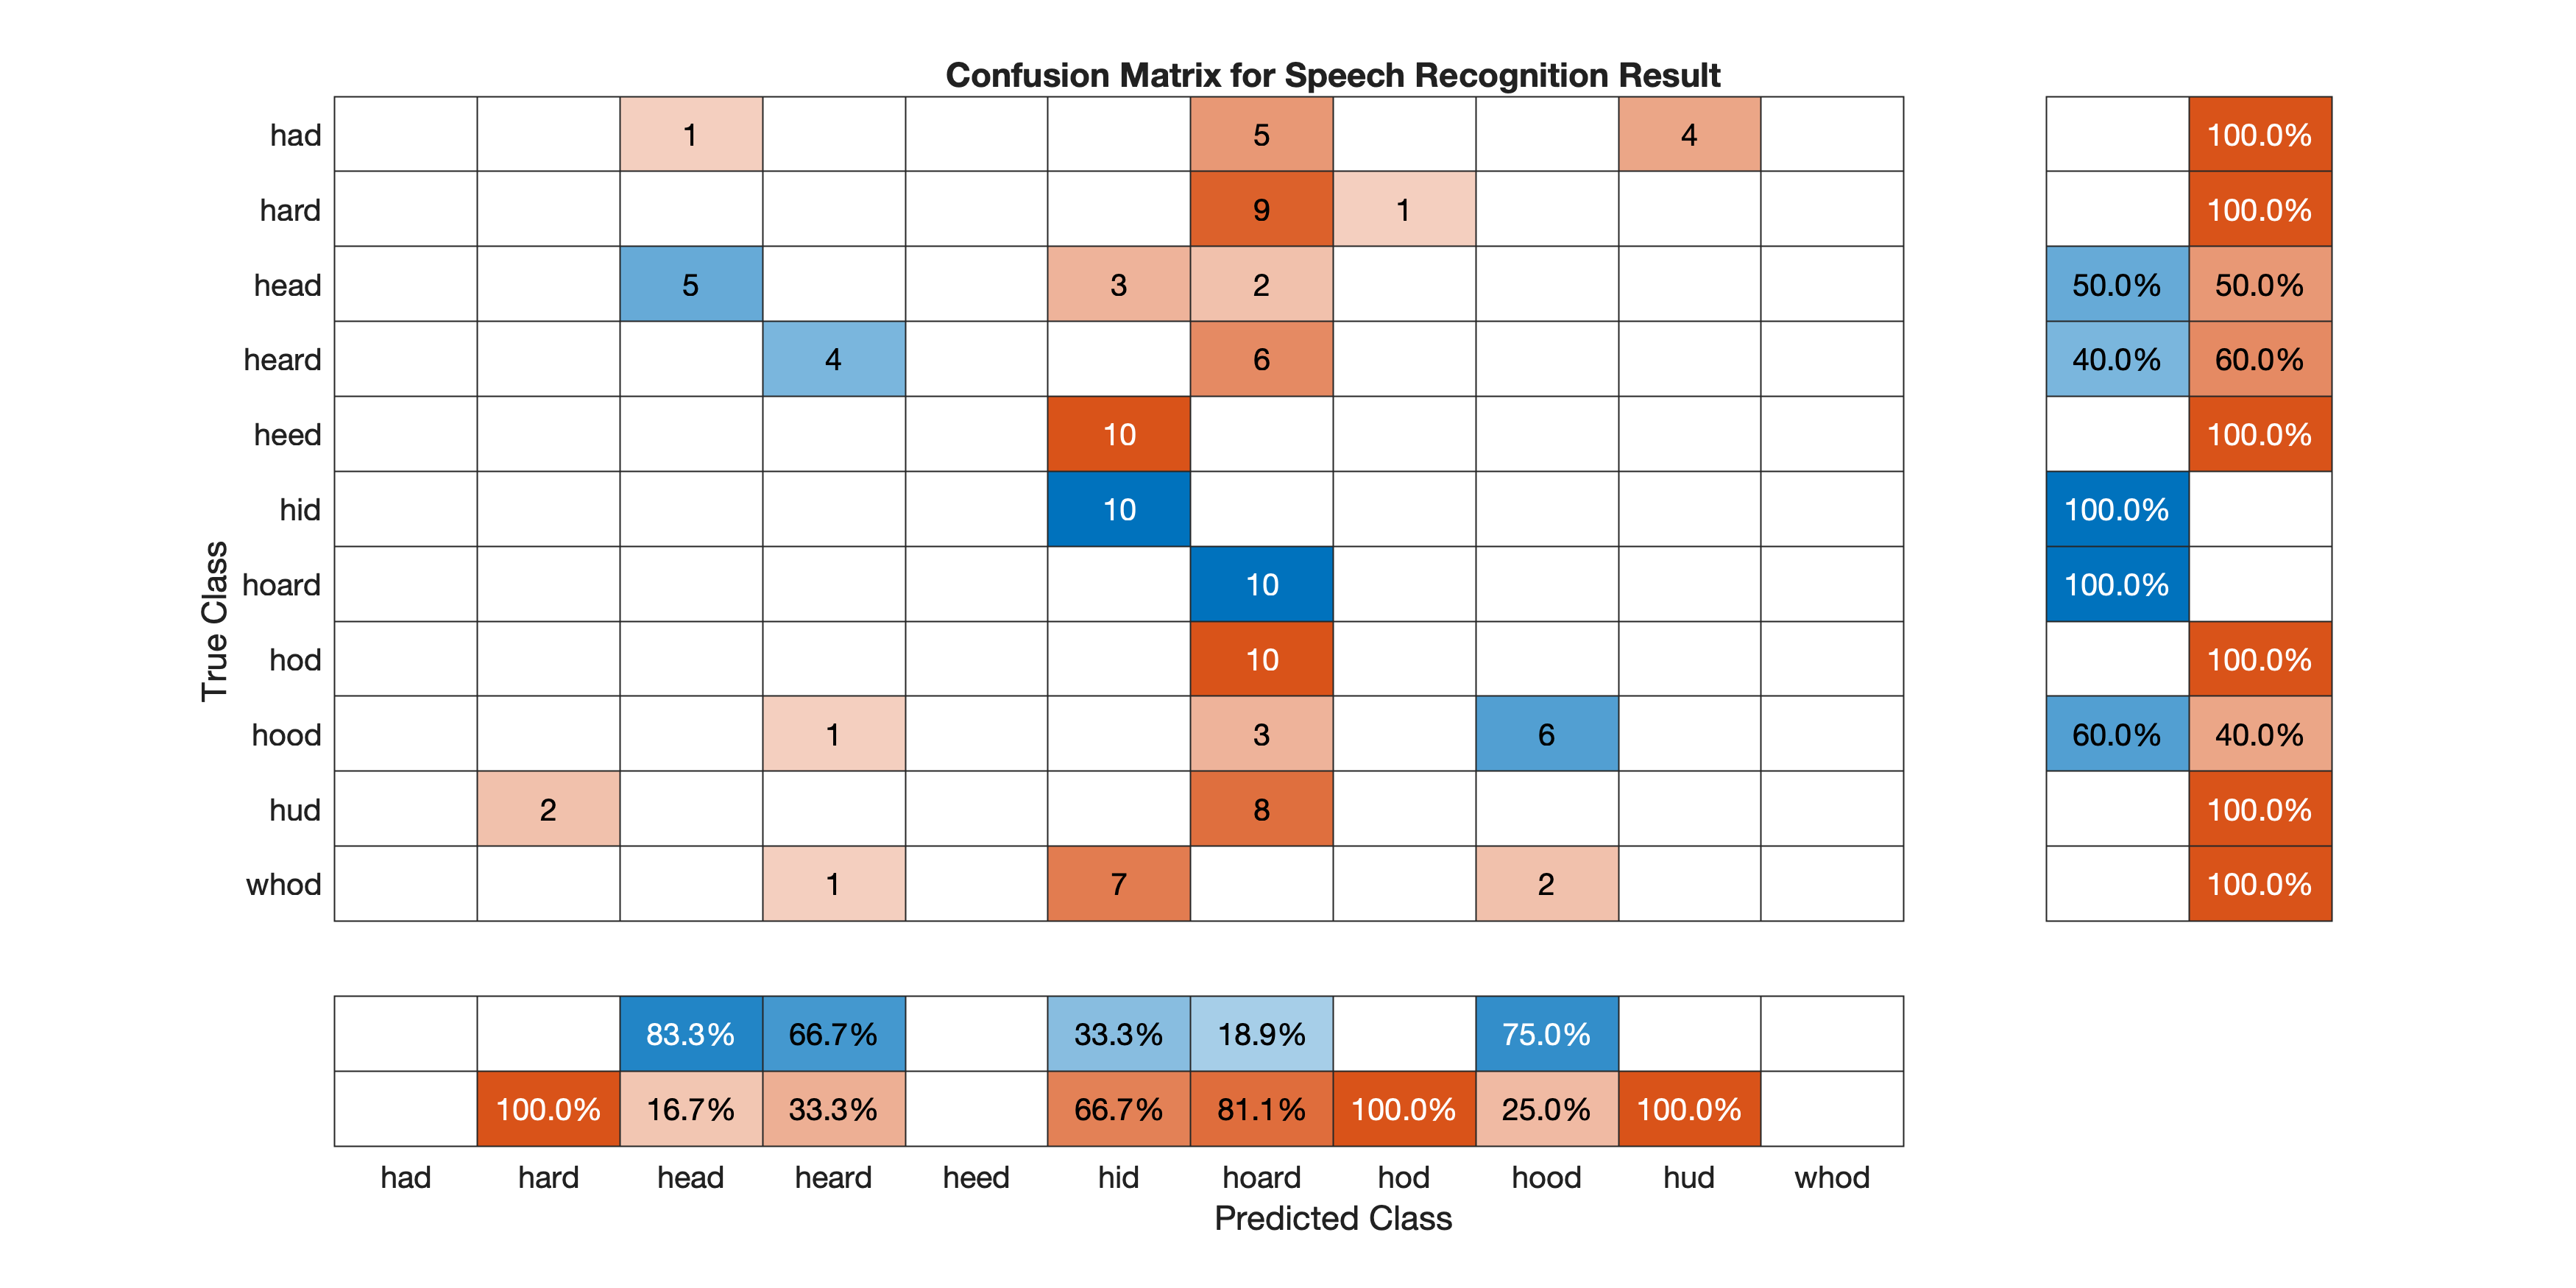
\includegraphics[width=\textwidth]{confusion_matrix}
\end{center}
\caption{\label{fig:confusion-matrix} Confusion matrix for HMM model training on the evaluation set.}
\end{figure}

\section{Data augmentation}

\paragraph{Characteristics of the validation data:}
The pronunciations in the validation dataset consist entirely of male voices across 11 groups of words.

\paragraph{Evaluation results of the validation data:}
\begin{itemize}
\item The prediction accuracy for “had” and “hard” is 0%.
\item The prediction accuracy for “heard” and “whod” is 10%.
\item The prediction accuracy for “hid” and “hoard” is relatively high, at 90\% and 100\% respectively.	
\end{itemize}

\paragraph{Augmentation measures for the Data:}
\begin{enumerate}
\item Train only on male voices.
\item Perform 3x or 5x repetition augmentation for male voice recordings.
\item Perform 3x or 5x repetition augmentation for audio samples of the words "had", "hard", "heard" and "whod".
\end{enumerate}

Following the application of data augmentation techniques, the resulting recognition outputs are evaluated using the optimal HMM model. The associated confusion matrix is presented in Figure \ref{fig:confusion-matrix-augmentation}.

\begin{figure}[h]
\begin{center}
\includegraphics[width=\textwidth]{confusion_matrix_data_augmentation}
\end{center}
\caption{\label{fig:confusion-matrix-augmentation} Confusion matrix for HMM model training on the data augmentation set.}
\end{figure}

\section{Conclusion}



%%%%%%%%%%%%%%%%%%%%%%%%%%%%%%%%%%%%%%%%%%%%%%%%%%%%%%%%%%%%%%%%%%%%%%%%%%%%%%

\newcommand{\doi}[1]{DOI: \href{http://dx.doi.org/#1}{\nolinkurl{#1}}}
\bibliographystyle{ieeetr}
\bibliography{refs}

%%%%%%%%%%%%%%%%%%%%%%%%%%%%%%%%%%%%%%%%%%%%%%%%%%%%%%%%%%%%%%%%%%%%%%%%%%%%%%

\end{document}
